
%(BEGIN_QUESTION)
% Copyright 2010, Tony R. Kuphaldt, released under the Creative Commons Attribution License (v 1.0)
% This means you may do almost anything with this work of mine, so long as you give me proper credit

Operators determine a control valve has a problem, because the stem is found to be at the 30\% position when the loop controller is set to output 50\% in manual mode.  A technician goes to this valve to diagnose the problem, and begins by connecting his multimeter to the circuit as shown:

$$\includegraphics[width=15.5cm]{i00748x01.eps}$$

The moment he connects his multimeter to the valve positioner's signal terminals, the valve closes fully and the multimeter reads 9.83 milliamps.

\vskip 10pt

Based on this information, determine where the most likely location of the fault is: in the {\it loop controller}, the {\it signal wiring}, the {\it positioner}, or the {\it actuator}.  Also, critique the technician's diagnostic strategy -- would you have done a different test?

\vskip 20pt \vbox{\hrule \hbox{\strut \vrule{} {\bf Suggestions for Socratic discussion} \vrule} \hrule}

\begin{itemize}
\item{} If you were the technician and did not have any test equipment on your person such as a multimeter, how would you test the valve?  Identify some sources of information available on this valve (with no test equipment) useful for diagnosing the problem.
\end{itemize}

\underbar{file i00748}
%(END_QUESTION)





%(BEGIN_ANSWER)

The glaring mistake in the technician's test is that he connected an ammeter in {\it parallel} when he should have connected it in {\it series}.  

%(END_ANSWER)





%(BEGIN_NOTES)

As it stands, this one test doesn't tell us much except that the controller is not at fault, and that the wiring is likely not at fault.

\vskip 10pt

The reason the ammeter does not register 12 mA (equivalent to 50\%) is because the ammeter's parallel connection with the positioner forces current to split between the two, so the ammeter is not sensing the full current output by the controller.

\vskip 10pt

Given that the percentage equivalent of 9.83 mA in a 4-20 mA range exceeds the valve stem's position of 30\%, we may safely conclude this is not the controller's fault.  If so, the measured current would be no more than 8.8 mA (30\%).  A wiring fault is also unlikely because that would most likely take the form of either an open or a short, in which case the measured current would be practically zero.

%INDEX% Final Control Elements: troubleshooting

%(END_NOTES)


